\documentclass[10pt]{article}

\usepackage[margin=2.5cm]{geometry}
\usepackage{graphicx}
\usepackage{listings}
\usepackage{xpatch}
\usepackage{color}
\usepackage{amsmath}
\usepackage[spanish]{babel}
\usepackage{url}

\begin{document}
	{	\centering
		\scshape
		\LARGE
		Universidad de los Andes
		
		\large
		Departamento de F\'isica
		
		\vspace{1cm}
		
		Propuesta de Proyecto Microscop\'ia Moderna
		
		Microsc\'opio de escaneo laser
		
		\normalsize
		Juan Barbosa
		
	}
	
	\section{Introducci\'on}		
		La microscop\'ia de escaneo laser es una t\'ecnica de microscop\'ia en la cual se hace incidir luz sobre una peque\~na parte de un objeto, y se cuantifica la reflexi\'on de la misma. En ese sentido hace parte de las t\'ecnicas de luz reflejada. Dado que el punto donde se concentra la luz es relativamente peque\~no respecto a el tama\~no de la muestra, es necesario samplear la reflexi\'on en los ejes $x$ y $y$.
		
		Experimentalmente la parte \'optica se compone de un \textit{beam splitter} y uno o m\'as lentes para enfocar el haz de luz.
		
		\begin{figure}[h]
			\centering
			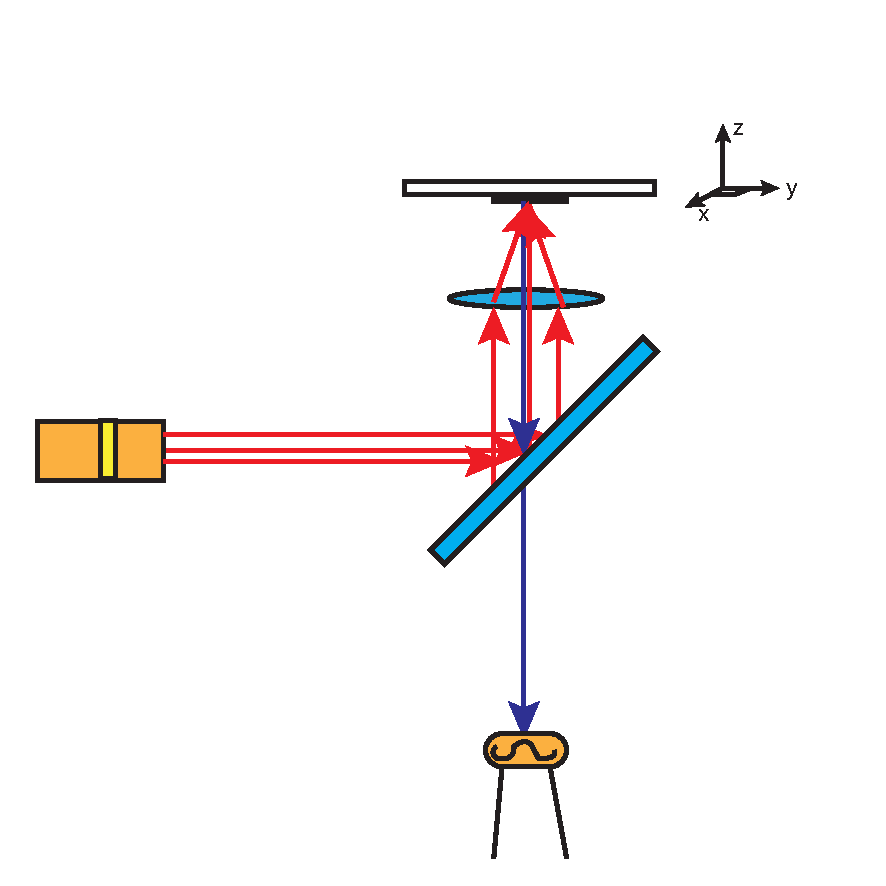
\includegraphics[width=0.35\linewidth]{beam.pdf}
			\caption{El haz de luz proveniente del laser, se refleja y se enfoca usando un lente. El rayo incide sobre la muestra, y la luz reflejada es captada por un detector.}
		\end{figure}
	
	\section{Objetivos}
		\begin{enumerate}
			\item Construcci\'on de un microsc\'opio de escaneo laser usando materiales de f\'acil acceso comercial.
			\item Adquirir datos con diferentes muestras.
			\item Mantener el presupuesto bajo, la electr\'onica s\'imple y el c\'odigo legible. Se espera que el proyecto a futuro sirva de forma pedag\'ogica, para las ciencias computacionales y la electr\'onica.
		\end{enumerate}
	
	\section{Metodolog\'ia}
		El sistema \'optico necesario para la implementaci\'on del proyecto se encuentra en su totalidad contenida en los m\'odulos de lectura (y escritura) de medios digitales tales como CD, DVD y Blu-Ray. De estos tres sistemas el de menor longitud de onda es el Blu-Ray, sin embargo el sistema \'optico se encuentra minimizado, dificultando el acceso a las partes relevantes. Por esta raz\'on se opt\'o por el sistema \'optico de los CD's, los cuales ya se encuentran adquiridos y corresponden con la referencia \texttt{KSS-213B}.
		
		En estos sistemas se realizaron cambios de los l\'aseres infrarojos por rojos de acceso comercial local. La etapa de detecci\'on tambi\'en se modific\'o, sin embargo aun no se encuentra implementada en su totalidad, dado que por la intensidad de la se\~nales se espera que se deba agregar una etapa de amplificaci\'on. Estos sistemas cuentan con dos bobinas internas para controlar el enfoque ($z$) y el movimiento en una direcci\'on $x$ \'o $y$. Estos movimientos son lo suficientemente peque\~nos para seguir los datos grabados sobre la superficie de un cd ($\approx 1\mu$m). De los dos sistemas \'opticos con los que se cuenta, el primero tiene las funciones de enfoque y movimiento en $x$, mientras el otro s\'olo se mueve en $y$.
		
		El microsc\'opio en su interior cuenta con un microcontrolador \texttt{Atmega 328}, el cual se encarga de realizar los movimientos en $x$ y $y$, obtener los datos y enviarlos por puerto USB a un computador usando un protocolo UART. Esta etapa ya se encuentra implementada. En el computador los datos son recibidos y graficados, al finalizar el projecto se espera contar con una libreria en Python para simplificar el acceso a los datos, sin perder de vista el hecho que el microsc\'opio ser\'a manejado con c\'odigo y no con una interfaz gr\'afica, esto con el objetivo de motivar la computaci\'on a nivel general.
		
		\begin{figure}[h]
			\centering
			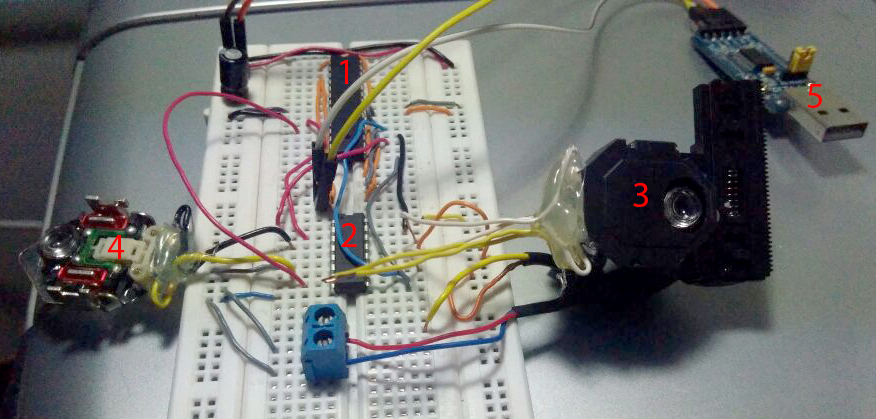
\includegraphics[width=0.7\linewidth]{breadboard.jpg}
			\caption{Circuito actual. (1) Microcontrolador. (2) Puente H, etapa de potencia para los motores. (3) Sistema \'optico principal con laser y movimiento en $x$. (4) Sistema \'optico con movimiento en $y$. (5) Comunicaci\'on UART.}
		\end{figure}
		
		\begin{figure}[h]
			\centering
			\begin{tabular}{cc}
				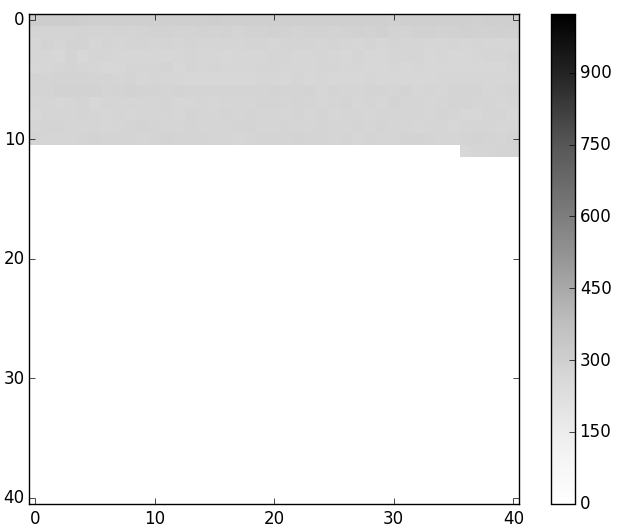
\includegraphics[width=0.3\linewidth]{data1.png} &
				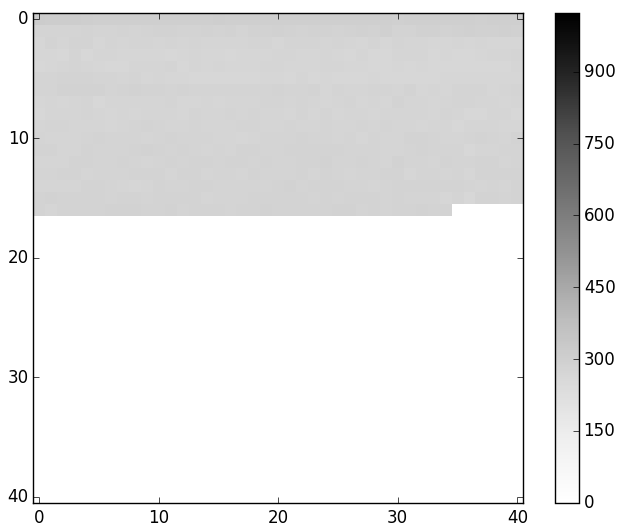
\includegraphics[width=0.3\linewidth]{data2.png}
			\end{tabular}
			\caption{Barrido, observado en el computador. La escala corresponde a 10-bits.}
		\end{figure}
	
	\nocite{*}
	\bibliography{Bib}
	\bibliographystyle{plain}
\end{document}